\chapter{Design}
The following chapter discusses the planning and design choices of the system. 

\section{Architectural Design} \label{sec:architecture}
Architectural design is concerned with understanding how a software system should be organized and designing the overall structure of that system \cite{sommerville}. Architectural design is the first stage in the software design process and is the critical link between design and requirements engineering, as it identifies the main structural components in a system and the relationships between them \cite{sommerville}. 

\begin{figure}[H]
    \centering
    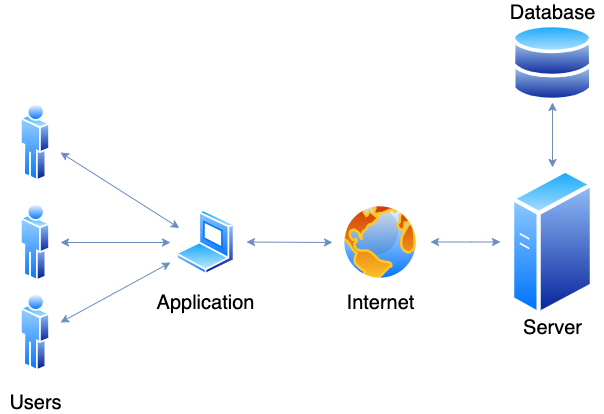
\includegraphics[width=0.8\textwidth]{7design/images/systemArchitecture.png}
    \caption{System architecture.}
    \label{fig:sysarchitecture}
\end{figure}

Figure \ref{fig:sysarchitecture} represents the system architecture of codeHelper. Users interact with the application which then makes calls, over the internet, to the server via HTTP requests or websocket communication. The server interacts with a database and serves information back the the client application.

\subsection{The Stack}

A technology stack is a combination of programming languages, frameworks, tools and technologies that are used to build and run an application. Figure \ref{fig:architecture} shows the architecture for the `codeHelper' stack. 

\begin{figure}[H]
    \centering
    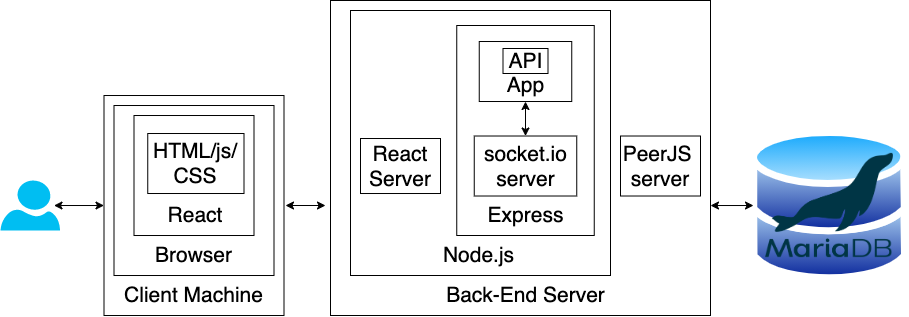
\includegraphics[width=\textwidth]{7design/images/architecture.png}
    \caption{Stack architecture with React.}
    \label{fig:architecture}
\end{figure}

Figure \ref{fig:architecture} shows that React, the API express application, socket.io (websocket) and PeerJS are all running on the same server. Due to the scale of the project, and resources provided by the School, this was the simplest way to deploy the codeHelper system. However, the modular separation of these components means that it would be straightforward to deploy them all on separate servers. Distributing network traffic across multiple servers would help to reduce demand on each individual server, as a result of which the request response time and availability of the application improves. Additionally, distributing the services can help to ensure performance and reliability of computing resources, both physical and virtual as well as adding redundancy and resilience to computing environments \cite{ibmload}.

\subsubsection{ReactJS}\label{sec:designreact}

ReactJS, commonly referred to as React, is a front-end framework. It is a JavaScript library which is deployed to develop reusable user interface (UI) components. It was selected for this project because of its performance, popularity and manageable learning curve \cite{Aggarwal}.

React enables development of large and complex single page web applications - meaning that it can change data and display without entire page refreshes. React implements a Model-View-Controller pattern \cite{Aggarwal}, shown in Figure \ref{fig:mvcreact}.

\begin{figure}[H]
    \centering
    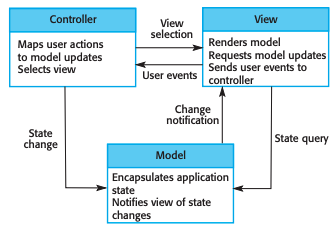
\includegraphics[width=0.5\textwidth]{7design/images/mvc.png}
    \caption{\gls{mvc} pattern \cite{sommerville} used by ReactJS.}
    \label{fig:mvcreact}
\end{figure}

One of the key features of React is its implementation of a `Virtual DOM' \cite{Aggarwal}. The virtual DOM is similar to the one which is generated by the browser, however React stores it in memory. This allows react to consider any requests for change to the page content in a different way than the browser would. When a request to change the page content is made, React makes the change to the virtual DOM and then compares it to the existing DOM in the browser to find differences. React then only rerenders the components of the page that differ between the virtual DOM and actual DOM providing a large boost to the performance of the application \cite{Aggarwal}.

React is, by default and in this project, a client side rendering application as shown in \ref{fig:csr}. This means that data is processed on both the client and server. The initial page load is relatively slow, however subsequent page loads are a lot faster since the server only needs to post requests for getting run time data. Additionally, the entire UI does not need to be downloaded from the server after each change \cite{csr}. Reconfiguring React to render on the server side would increase data security, make processing performance more predictable across the varying student machines/networks and minimise browser compatibility issues \cite{ssr}. For the codeHelper system, React was rendered on the client side to reduce load on the server and to minimise page load time.

\begin{figure}[H]
    \centering
    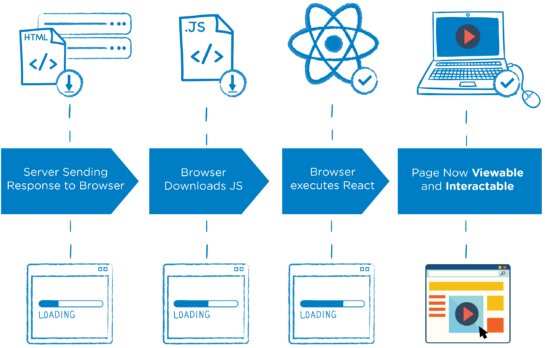
\includegraphics[width=0.7\textwidth]{7design/images/csr.png}
    \caption{Client side rendering process for ReactJS \cite{csr}.}
    \label{fig:csr}
\end{figure}

\subsubsection{Node.js}

Node.js is an asynchronous event-driven, open-source, cross-platform, back-end JavaScript runtime environment designed to build scalable network applications \cite{node}.

Since Node.js uses Javascript in the backend, it means Javascript is used across the entire stack (other than SQL). This, unifies the language and JSON data format and enables resources to be reused across the stack. It was selected for use in this project because of its popularity, performance and because of previous experience.

Another advantage of Node.js is \gls{npm}. This is installed by default with Node.js which provides a collection of publicly available, reusable libraries which are installed and used easily in Node applications.

\subsubsection{Express}\label{sec:express}

Express.js is a Node.js framework. Its purpose is to reduce repetition of code and simplify API development by simplifying the handling of routing and middleware. Without Express, tasks such as handling the details of payload, cookies and session storage would have to be done manually. It was selected for this project because of its popularity, simplicity and previous experience.

\subsubsection{MariaDB}\label{sec:stackdb}

The choice of a \gls{sql} (relational) database is justified in section \ref{whysql}. MariaDB was selected for this project because it is the database used by the School. 

\section{Interface}\label{sec:interface}

First, this section defines Lauesen's usability factors \cite{lauesen}, a set of factors that capture the essentials of usability which were considered throughout the design of the system. Secondly, with these factors in mind, the section discusses the initial design of the system interface. Thirdly, the section discusses the final design of the system interface.

\subsection{Lauesen's Usability Factors}

Lauesen \cite{lauesen} outlines the following six usability factors:

    \paragraph{Fit for Use (\textit{or functionality})} The system can support the tasks that the user has in real life.
    
    \paragraph{Ease of Learning} How easy is the system to learn for various groups of users?
    
    \paragraph{Task Efficiency} How efficient is it for the frequent user?
    
    \paragraph{Subjective Satisfaction} How satisfied is the user with the system?
    
    \paragraph{Ease of Remembering} How easy is it to remember for the occasional user?
    
    \paragraph{Understandability} How easy is it to understand what the system does? This
    factor is particularly important in unusual situations, for instance error situations
    or system failures. Only an understanding of what the system does can help the
    user recover.

A focus on developing the application to be `fit for use' is the same as focusing on creating a system that allows users to complete the tasks outlined in the system requirements - the goal of this project. As a result, the `fit for use' factor is not discussed in the following section. 

\subsection{Wireframes}

This subsection shows the wireframes that were designed in the early stages of the project and discusses how Lauesen's usability factors were considered.  The interface was designed based on the requirements defined in chapter \ref{chap:req}. Wireframes were developed for a subset of the requirements, representing the core features of the system.

\subsubsection{Demonstrator}

Figure \ref{fig:demoTickets} shows a simple, coloured wireframe for the helpdesk page of the application. This is the main page for demonstrators and provides them a starting point for analysing live tickets. This page was loosely based on the Spiceworks helpdesk. It is designed to convey the basic information for all tickets for class demonstrators to scan, after which they can select a ticket from the bottom table and learn more. 

The help desk design, shown in figure \ref{fig:demoTickets}, targets the factors `Ease of Learning' and `Understandability' by using commonplace icons alongside a simple and conventional page layout.

The table displaying tickets, shown at the bottom of figure \ref{fig:demoTickets}, targets `task efficiency' and `subjective satisfaction' by focusing strongly on the workflow for demonstrators. It reduces the amount of information displayed to only what is necessary for a first scan of the live tickets - demonstrators begin on the help desk page, scan the live tickets and select a ticket. The option to begin a chat only appears once a ticket has been selected and, further, the option to begin a video chat appears only in that chat. This enables the workflow to be naturally reflected in the system and prevents the display from overwhelming instructors with too many options and too much information. 

The navbar shows the inclusion of a separate `messages' page. This allows demonstrators to efficiently handle multiple existing chats rather than accessing them individually on each ticket. This greatly improves task efficiency and subjective satisfaction, since demonstrators are able to multitask and complete more work in a much more natural way. 

\begin{figure}[H]
    \centering
    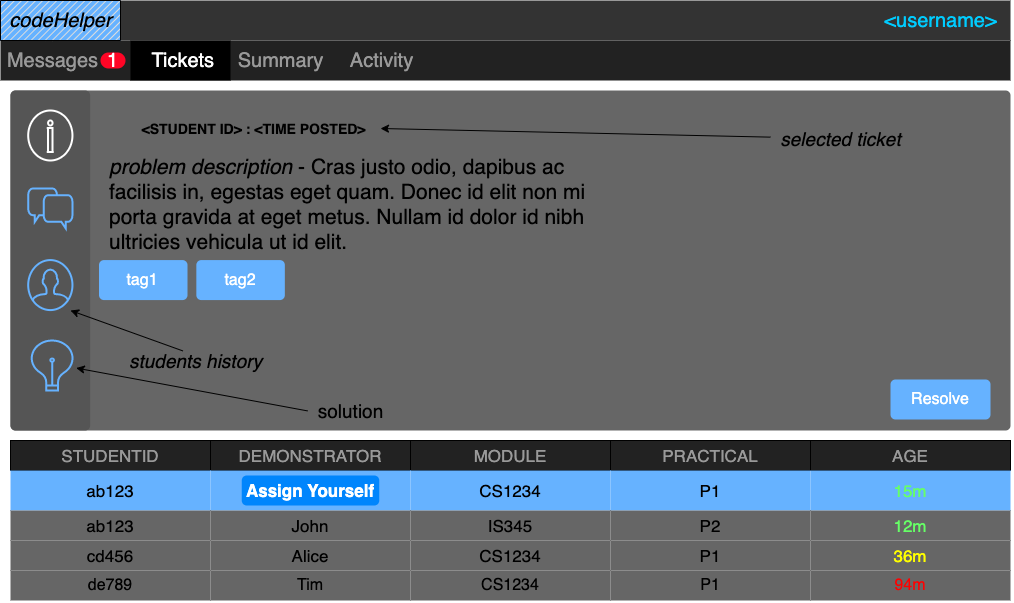
\includegraphics[width=\textwidth]{7design/images/revisedDemoTickets.png}
    \caption{Simple design for the demo ticket viewing interface.}
    \label{fig:demoTickets}
\end{figure}

Figure \ref{fig:demoActivity} shows a wireframe for the activity page. This page is loosely based on the Spiceworks helpdesk activity page. This page is designed to convey a timeline of activity that has occured on the application. This was implemented to allow lab leads and demonstrators to quickly scan recent activity to get information about ticket assignment, resolution and user registration at a glance. 

The page, shown in \ref{fig:demoActivity}, uses varying icons for the different activities. This is to emphasise the `understandability', `ease of learning' and `subjective satisfaction' of the page - since users are able to scan the recent activities quicker when looking at icons rather than text.

\begin{figure}[H]
    \centering
    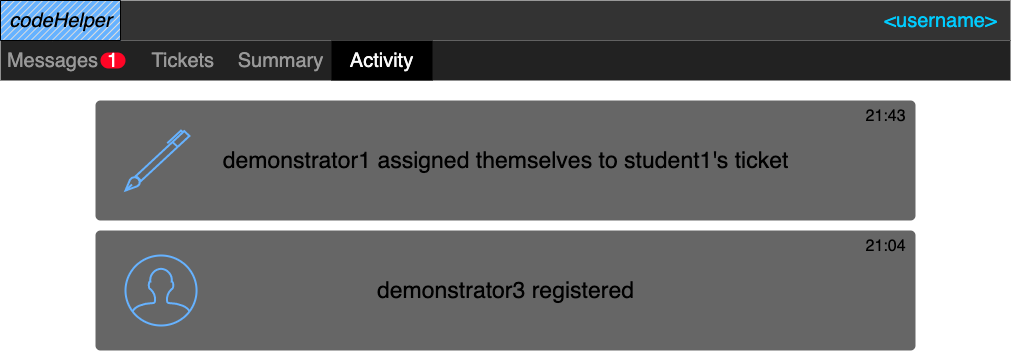
\includegraphics[width=\textwidth]{7design/images/activityDemo.png}
    \caption{Simple design for the activity viewing interface.}
    \label{fig:demoActivity}
\end{figure}

\subsubsection{Student}

The design for the student ticket posting page (show in figure \ref{fig:postTicket}) was based on the current system form (shown in figure \ref{fig:currentPostTicket}). This page is designed to allow students to post their ticket and is the first page that students see upon entering the application.

The page, shown in \ref{fig:postTicket}, considers usability `ease of learning', `understandability' and `task efficiency' by implementing an extremely simple form. The form contains inputs which describe exactly what information the user should provide at each input, minimising the potential for users to forget, misunderstand or misuse the ticket posting functionality of the application. 

\begin{figure}[H]
    \centering
    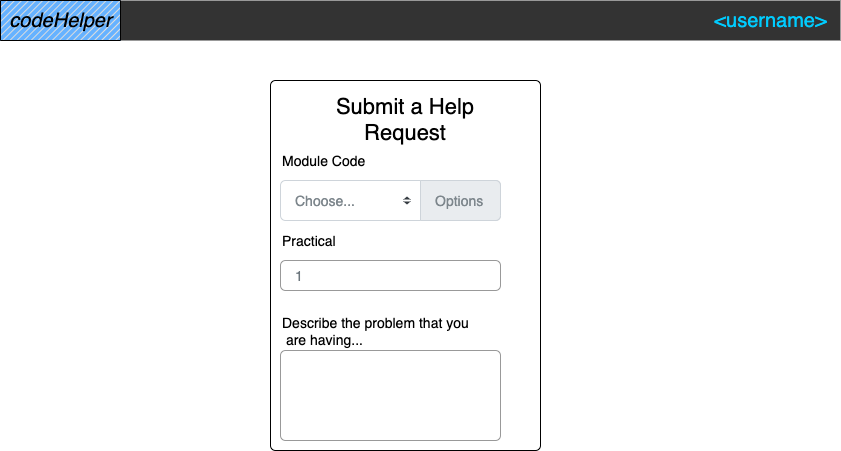
\includegraphics[width=0.8\textwidth]{7design/images/postTicket.png}
    \caption{Simple design for the student's ticket posting page.}
    \label{fig:postTicket}
\end{figure}

\begin{figure}[H]
    \centering
    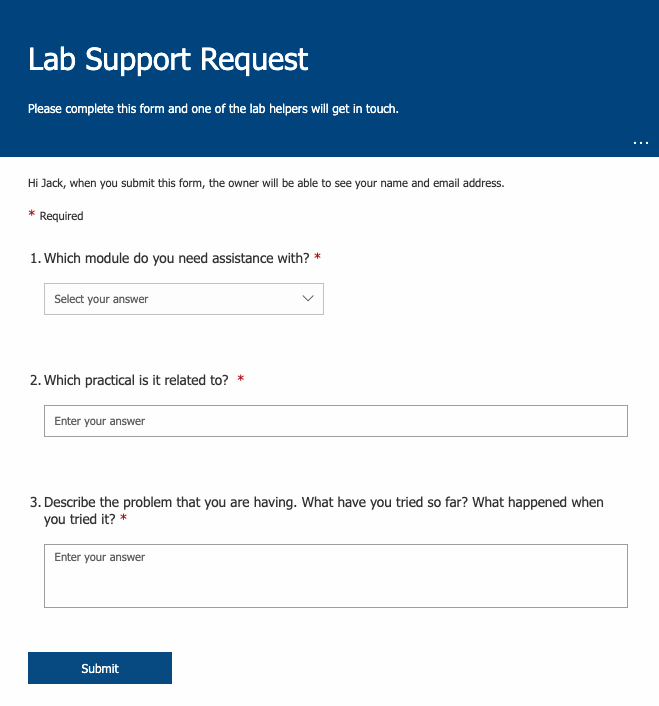
\includegraphics[width=0.7\textwidth]{7design/images/currentSystemForm.png}
    \caption{The current system's ticket posting form, implemented using Microsoft Forms.}
    \label{fig:currentPostTicket}
\end{figure}

After posting their ticket, students shall join a queue of users who have already posted tickets. The design for the ticket queue page is shown in figure \ref{fig:queuewire}. This was based loosely on the ClassroomQ design. 

The student aspect of the system consider usability by fixing the location of students in the application, assisting with each of Lauesen's factors. Student's location in the application is fixed based on their position in the workflow - for example, if a student has posted a ticket and is waiting in the queue, their view of the application is fixed on that page and they are unable to view the ticket posting form or live chat.

\begin{figure}[H]
    \centering
    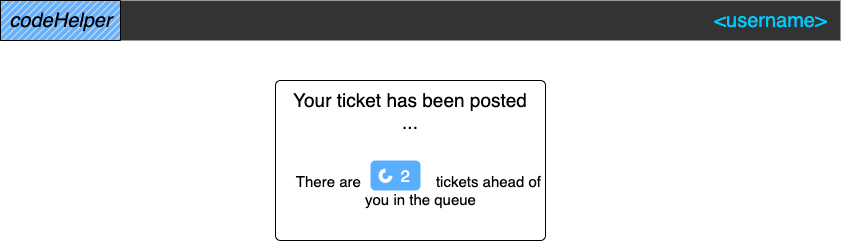
\includegraphics[width=0.8\textwidth]{7design/images/ticketQueue.png}
        \caption{Simple design for the student's ticket queue page.}
    \label{fig:queuewire}
\end{figure}

\subsubsection{Final Design}

The final design of the helpdesk page is shown in figure \ref{fig:helpdeskfinal}. The final design largely adheres to the original wireframe. A user avatar was added for satisfaction. The tag colour was also changed to allow a distinction between tags and the other buttons. Furthermore, a notification sound is played when a new message is received and a count of all unread messages is displayed in the navigation bar to notify demonstrators of new messages. 

\begin{figure}[H]
    \centering
    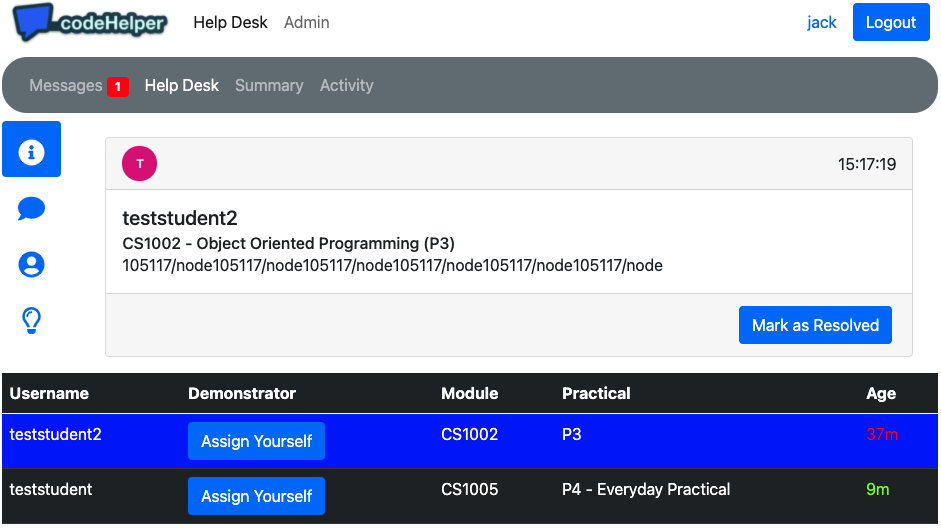
\includegraphics[width=\textwidth]{7design/images/helpdesk.png}
    \caption{Final helpdesk page design, where the demonstrator scans all tickets and selects one to investigate further and open communication with the student.}
    \label{fig:helpdeskfinal}
\end{figure}

As well as the use of conventional icons, tooltips were added to each button icon to improve usability - namely ease of learning, remembering and understandability. An example of a tooltip in the application is shown in figure \ref{fig:tooltip}. 

\begin{figure}[H]
    \centering
    
\includegraphics[width=0.3\textwidth]{7design/images/tooltip.png}
    \caption{Example of a tooltip in the application.}
    \label{fig:tooltip}
\end{figure}

If the user clicks on a tag in figure \ref{fig:helpdeskfinal}, a modal pops up showing all other tickets with that tag. This increases functionality, satisfaction and efficiency of the application by allowing demonstrators to investigate similar tickets. This improves usability by focusing on task efficiency and subjective satisfaction - demonstrators do not need to leave the main help desk to analyse past tickets. An example is shown in figure \ref{fig:tagModal}.

\begin{figure}[H]
    \centering
    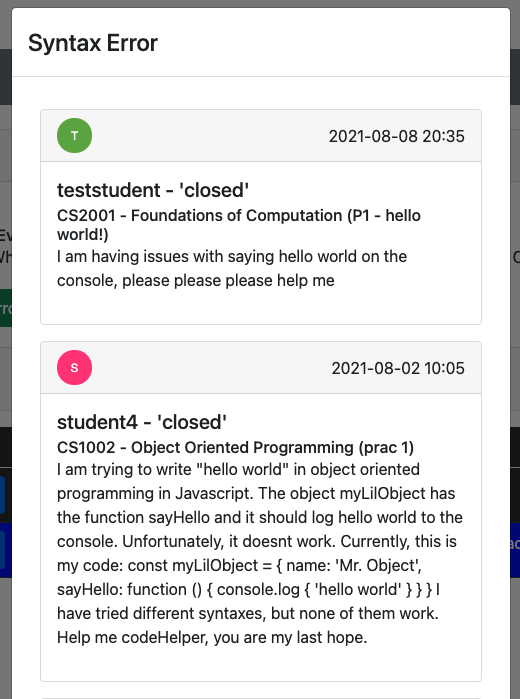
\includegraphics[width=0.5\textwidth]{7design/images/tagModal.png}
    \caption{Tag modal, where the demonstrator can investigate previous tickets with the same tag.}
    \label{fig:tagModal}
\end{figure}

The ticket form's final design is shown in figure \ref{fig:ticketForm}. The module code options are taken from the database, which contains all CS modules for years one and two. Additionally, lab leads can add or remove modules on the admin page.

\begin{figure}[H]
    \centering
    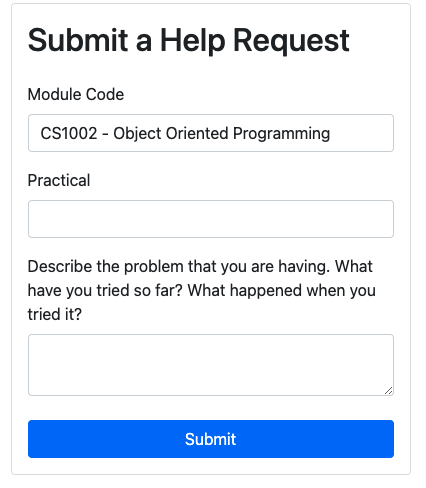
\includegraphics[width=0.5\textwidth]{7design/images/ticketForm.png}
    \caption{The ticket form, where a student can create a ticket about an issue they are having.}
    \label{fig:ticketForm}
\end{figure}

The activity page's final design is shown in figure \ref{fig:activity}. The page is much like the initial wireframe design, however includes colour coding of the icons to further improve usability - namely the task efficiency and ease of understanding. 

\begin{figure}[H]
    \centering
    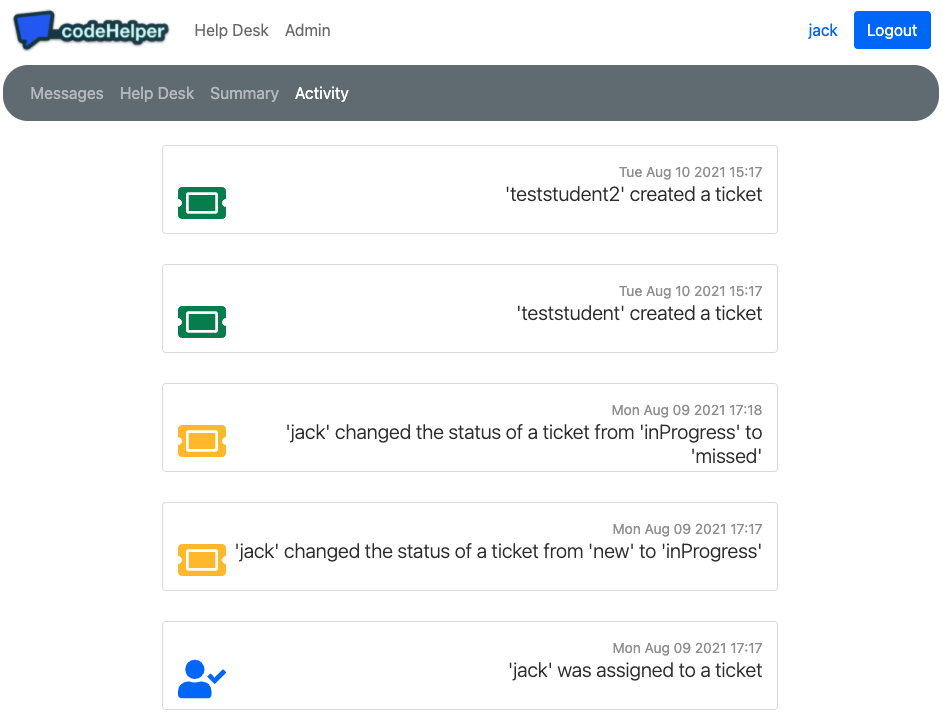
\includegraphics[width=0.9\textwidth]{7design/images/activity.png}
    \caption{The activity page, where a demonstrator can scan recent activity on the application.}
    \label{fig:activity}
\end{figure}

Figure \ref{fig:queue} shows the final design of the ticket queue component. It is the same as was planned in the wireframe.

\begin{figure}[H]
    \centering
    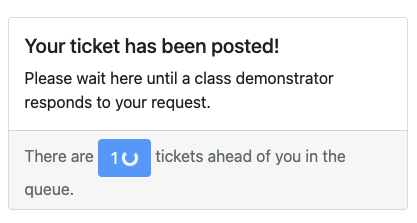
\includegraphics[width=0.5\textwidth]{7design/images/queue.png}
    \caption{The student queue page, where a student waits until a demonstrator assigns themselves to their ticket.}
    \label{fig:queue}
\end{figure}

Another aspect of the system that was added for usability was confirmation modals. Modals of this kind exist in various aspects of the system, such as when marking a ticket as resolved or attempting to close a lab. By asking for confirmation, they ensure that the user knows what action they are taking - helping to improve understandability and ease of remembering. An example is shown in figure \ref{fig:confmodal}.

\begin{figure}[H]
    \centering
    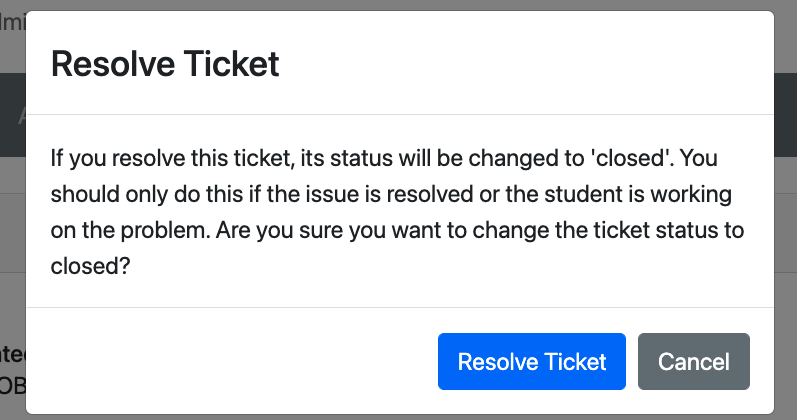
\includegraphics[width=0.6\textwidth]{7design/images/closeTicketModal.png}
    \caption{The student queue page, where a student waits until a demonstrator assigns themselves to their ticket.}
    \label{fig:confmodal}
\end{figure}

Further, modals were added in the final design to reflect changes in students queue position. These were added a result of feedback from the experiment, discussed in section \ref{sec:experiment}. The system originally redirected students to the ticket form page if the lab was closed or their ticket was resolved, providing no information. The experiment identified an area of usability that could be improved, and information modals were added to improve understandability. An example of one such modal, for when the lab is closed, is shown in figure \ref{fig:labclosedmodal}.

\begin{figure}[H]
    \centering
    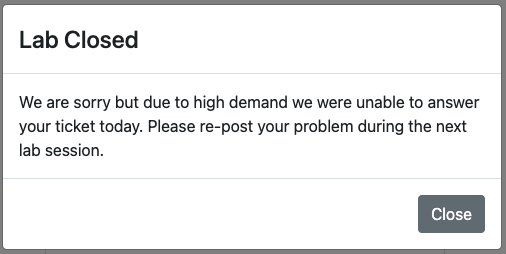
\includegraphics[width=0.6\textwidth]{7design/images/labClosedModal.png}
    \caption{The lab closed modal, shown to students when a lab is closed if they are queuing or in a chat with a demonstrators.}
    \label{fig:labclosedmodal}
\end{figure}

\subsection{Responsive Design}

Responsive Web Design is a set of strategies used to display web pages on screens of varying sizes. For this application, responsive web design was implemented and a Mobile-first design philosophy was primarily used.

Mobile-first is a philosophy of design which aims to improve user experience by considering mobiles first. The strategy comes from the concept of progressive advancement, meaning that design begins with how the codeHelper application looks on a mobile and then consider desktop computers after that. As a result of the limited real estate on a small mobile screen, considering the mobile view first forces us to prioritise the most important aspects of the application. When the application design is considered for desktop, the user experience will be improved as a result of this prioritisation \cite{mobilefirst}. 

Additionally, the usefulness of the application increases if it is designed for mobile use as a result of the fact that users are more often able to access the application. Students and demonstrators are able to chat, call and perform all other functionality `on-the-go' by using mobile devices.

Figures \ref{fig:mobStudChat} to \ref{fig:mobDemActiv} show how the application renders various pages on the application on an iPhone 6/7/8.

\begin{figure}[H]
    \centering
    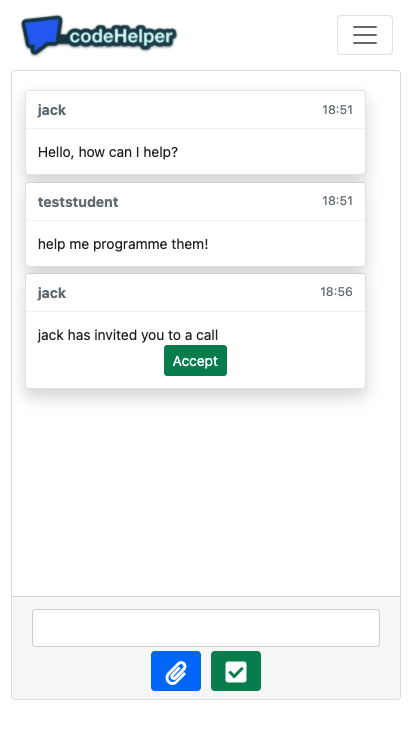
\includegraphics[width=0.5\textwidth]{8implementation/images/mobStudChat.png}
    \caption{Mobile view of student chat.}
    \label{fig:mobStudChat}
\end{figure}

\begin{figure}[H]
\centering
\begin{minipage}{.5\textwidth}
  \centering
    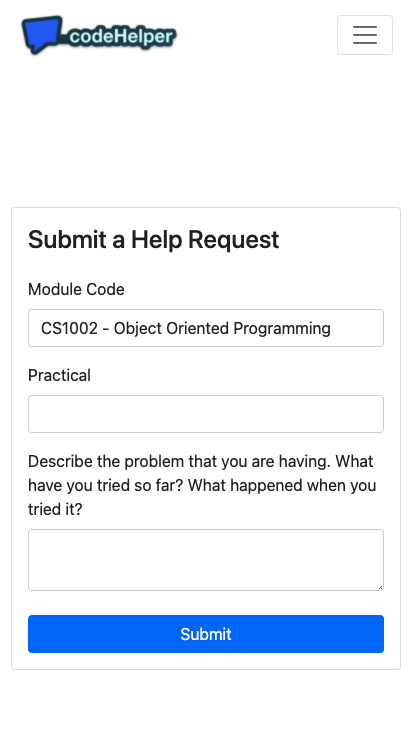
\includegraphics[width=\textwidth]{8implementation/images/mobStudForm.png}
  \captionof{figure}{Mobile view of student ticket\\ posting page.}
  \label{fig:mobStudForm}
\end{minipage}%
\begin{minipage}{.5\textwidth}
  \centering
    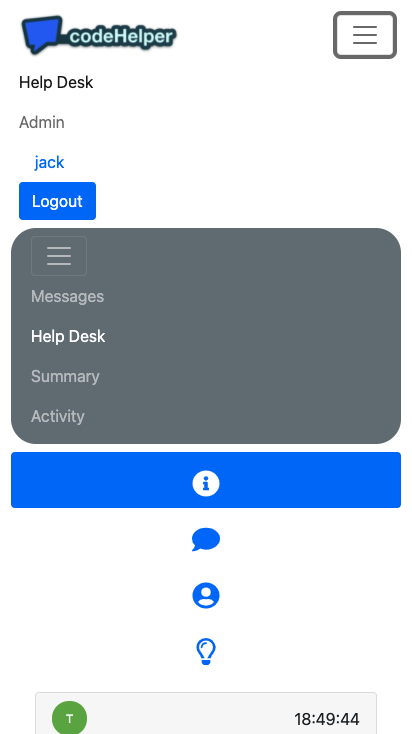
\includegraphics[width=\textwidth]{8implementation/images/mobDemNav.png}
  \captionof{figure}{Mobile view of demonstrator and main navigation bars.}
  \label{fig:mobDemNav}
\end{minipage}
\end{figure}

\begin{figure}[H]
\centering
\begin{minipage}{.5\textwidth}
  \centering
  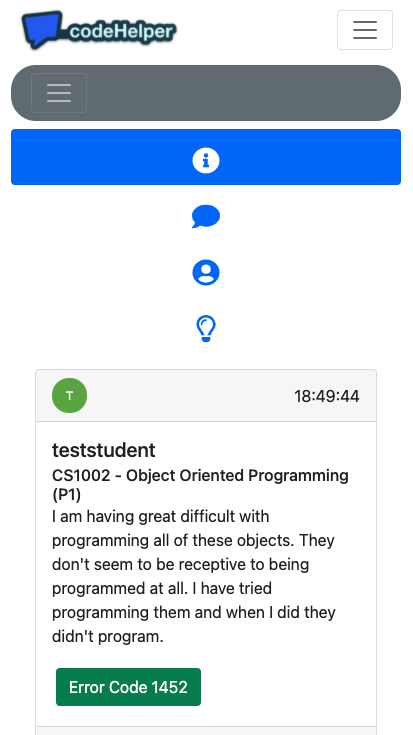
\includegraphics[width=\linewidth]{8implementation/images/mobDemDesk.png}
  \captionof{figure}{Mobile view of demonstrator \\ helpdesk.}
  \label{fig:mobDemDesk}
\end{minipage}%
\begin{minipage}{.5\textwidth}
  \centering
  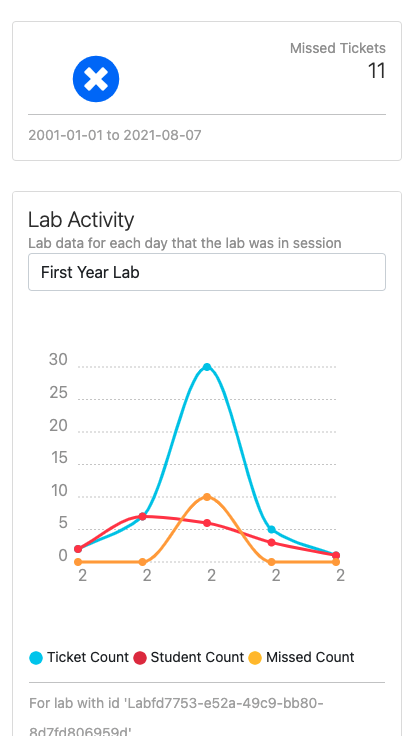
\includegraphics[width=\linewidth]{8implementation/images/mobDemActiv.png}
  \captionof{figure}{Mobile view of lab lead activity page.}
  \label{fig:mobDemActiv}
\end{minipage}
\end{figure}

One thing to note is that the video call page (accessed by starting a video call in a regular chat) does not render neatly on mobile. Although the page is still usable, it does not offer a similar level of experience to other pages. Full screen video chat is offered by default, although this does not work with the application as text chat and file sharing are not useable. Future work on this area would be needed if it was something that the customer felt was useful for a production system.

\newpage
\section{Database}

The E-R model is very useful in mapping meanings and interactions of real world enterprises onto a conceptual schema. The E-R data model employs three basic concepts: entity sets, relationship sets, and attributes \cite{db}. This section outlines a representation of the data in terms of entities, attributes and relationships between entities.

\subsubsection{Entities}\label{sec:entities}

The components of the systems are represented as the entities in table \ref{tab:er}.

\FloatBarrier
\begin{table}[H]
\centering
\begin{tabular}{ |l|c| } 
 \hline
 \textbf{Entity Set} & \textbf{Attributes}\\ 
 \hline
  user & \underline{username}, name\\ 
 \hspace{6pt}user.student & \\ 
 \hspace{6pt}user.demonstrator & \\
 \hspace{12pt}user.demonstrator.labLead & \\
 \hline
 auth & \underline{username}, password, role \\
 \hline
 ticket & \underline{ticketId}, issueDescription,\\
 & practical, resolutionStatus \\
 \hline
 lab & \underline{labId}, status\\
 \hline
 solution & \underline{solutionId}, solutionDescription\\
 \hline
 tag & \underline{name} \\
 \hline
 module & \underline{moduleCode}, name \\
 \hline
 activity & \underline{id}, type \\
 \hline
\end{tabular}
\caption{Table of entities and associated attributes.}
\label{tab:er}
\end{table}
\FloatBarrier

Primary keys are denoted as \underline{underlined}. %Foreign keys are denoted in \textit{italics}.

Note that \textbf{user.student} and \textbf{user.demonstrator} are disjoint specialisations of the entity set \textbf{user} - a user is always a student or demonstrator (or specialisation of demonstrator). \textbf{user.demonstrator.labLead} is a further specialisation of \textbf{user.demonstrator}, not disjoint. 

\subsubsection{Relationships}\label{sec:relationship}
The relationships between entities, and the constraints on them, are defined in this section. 

\FloatBarrier
\begin{table}[H]
\centering
\begin{tabular}{ |c|c|c|c| } 
 \hline
 \textbf{Relationship} & \textbf{Entities} & \textbf{Participation} & \textbf{Cardinality}\\ 
 \hline
 $r$ & $e_1$, $e_2$ & total, partial & M-1 \\
 \hline
\end{tabular}
\caption{Example table row, showing participation and cardinality for a relationship between two entities.}
\label{tab:er2}
\end{table}
\FloatBarrier 

Many is denoted as M, one as 1 such that one to many relationship would be denoted 1-M. Note that for a relationship $r$ that is many (in $e_1$) to one (in $e_2$) and has total participation from $e_1$ but partial from $e_2$ then the row in the table \ref{tab:er3} is written as shown in the example table row in \ref{tab:er2}. Participation will be listed in order that entities are written.

\FloatBarrier
\begin{table}[htbp]
\centering
\resizebox{\columnwidth}{!}{\begin{tabular}{ |c|c|c|c|c| } 
 \hline
 \textbf{Relationship} & \textbf{Relationship Attributes} & \textbf{Entity Sets} & \textbf{Participation} & \textbf{Cardinality}\\ 
 \hline
 creates & creation\_timestamp & user.student, ticket & partial, total & 1-M \\
 assignedTo & demAssigned\_timestamp & user.demonstrator, ticket & partial, partial & 1-M\\
 writes & demSolved\_timestamp & user.demonstrator, solution & partial, total & M-M\\
 leads & & user.demonstrator.labLead, module & partial, total & 1-M\\
 postedIn &  & ticket, lab & total, partial & M-1\\
 hasTicketTag & & ticket, tag & total, partial & M-M\\
 regarding && ticket, module & total, partial & M-1\\
 toDoWithSolution & & activity, solution & partial, total & 1-M\\ 
 toDoWithTicket & & activity, ticket & partial, total & 1-M\\
 did & & activity, user & total, total & M-1\\
 hasAuth && user, auth & total, total & 1-1 \\ 
 \hline
\end{tabular}}
\caption{Table showing entities, relationships between, relationship attributes, participation and cardinality.}
\label{tab:er3}
\end{table}
\FloatBarrier

\subsubsection{Entity Relationship Diagram}\label{sec:er}

Figure \ref{fig:ER} shows an entity relationship diagram for the database, comprised of the entities and relationship discussed in section \ref{sec:entities} and \ref{sec:relationship}.

An entity set is represented in an E-R diagram by a rectangle, which is divided into two parts. The first part, which is shaded blue, contains the name of the entity set. The second part contains the names of all the attributes of the entity set. A relationship set is represented in an E-R diagram by a diamond, which is linked via lines to a number of different entity sets (rectangles) \cite{db}. 

\begin{figure}[H]
    \centering
    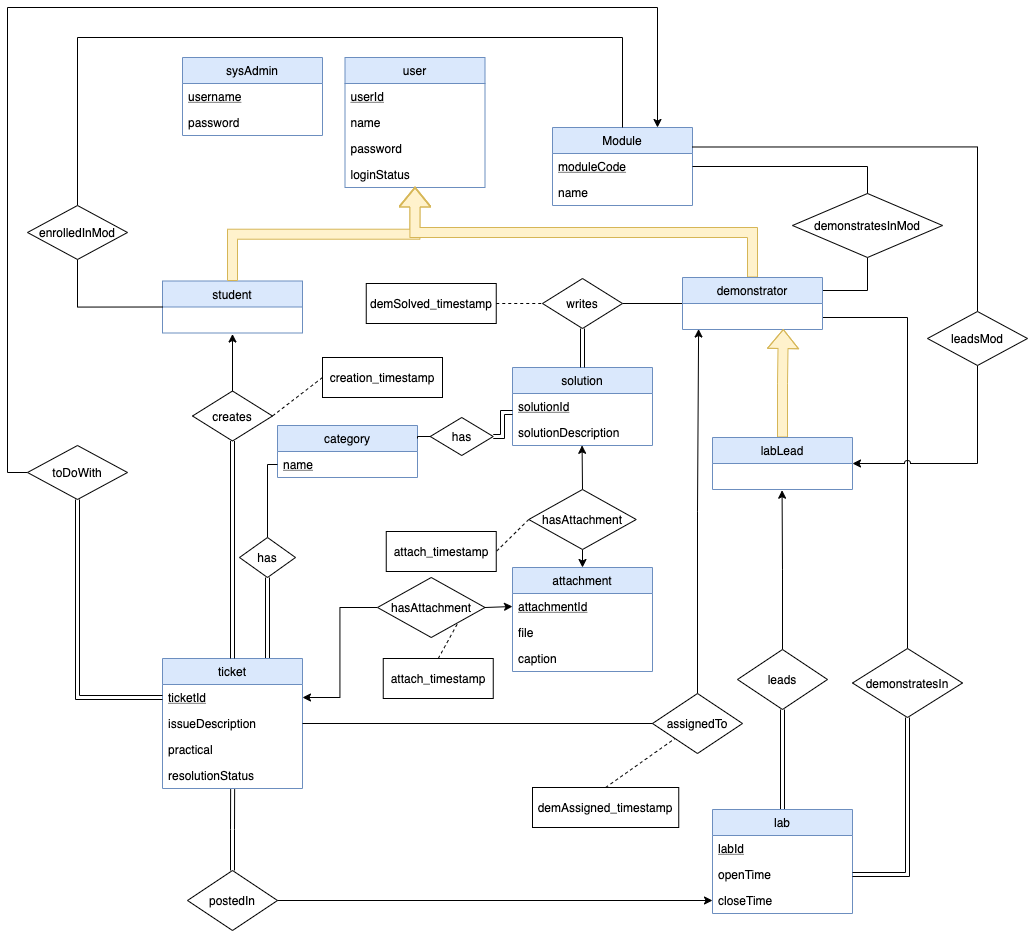
\includegraphics[width=\textwidth]{7design/images/ER.png}
    \caption{\gls{er} diagram for the system.}
    \label{fig:ER}
\end{figure}

\subsubsection{Relational Schema}\label{sec:relschem}

This section defines a database schema based on the ER model that was derived in section \ref{sec:er}. Below, and shown diagramatically in figure \ref{fig:relationalschema}, is a relational schema which is mapped to from the ER diagram (shown in figure \ref{fig:ER}) and its constraints.  

\noindent student - \underline{\textit{username}}, name \\
demonstrator - \underline{\textit{username}}, name \\
labLead - \underline{\textit{username}}, name \\
auth - \underline{username}, password, role \\
ticket - \underline{id}, issueDescription, \textit{moduleCode}, practical, resolutionStatus, \textit{studentUsername}, creation\_timestamp, close\_timestamp, \textit{demonstratorUsername}, demAssigned\_timestamp, \textit{labId}, \textit{solutionId} \\
tag - \underline{name} \\
solution - \underline{id}, title, solutionDescription, \textit{demonstratorUsername}, creation\_timestamp\\
lab - \underline{labId}, title, status\\
hasTicketTag - \underline{\textit{tickedId}}, \underline{\textit{name}}\\
module - \underline{moduleCode}, name, \textit{labLead.username}\\
activityRecord - \underline{id}, type, \textit{username}, \textit{ticketId}, \textit{solutionId}, resolutionStatusTo, resolutionStatusFrom, creation\_timestamp \\

\subsubsection{Relational Schema Diagram}

Figure \ref{fig:relationalschema} shows a diagram for the relational schema which is defined in section \ref{sec:relschem}.

\begin{figure}[H]
    \centering
    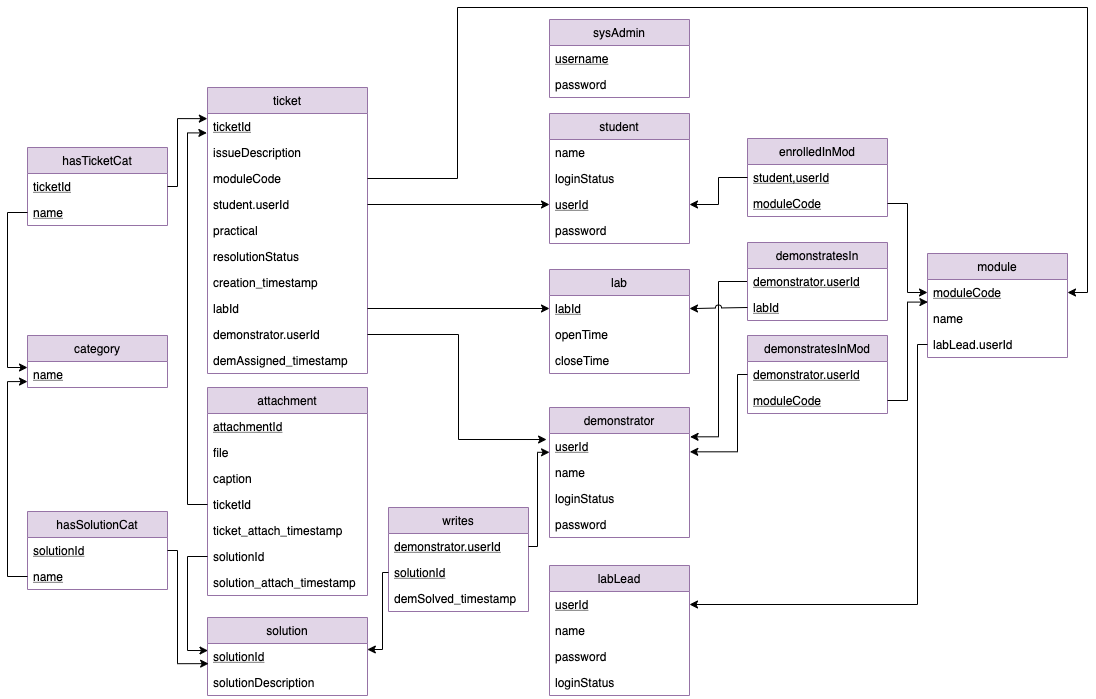
\includegraphics[width=0.7\textwidth]{7design/images/relationalSchema.png}
    \caption{Relational schema diagram for the system.}
    \label{fig:relationalschema}
\end{figure}

\subsection{Design Choices}

\subsubsection{SQL vs NoSQL}\label{whysql}

SQL databases are relational databases, named after Structured Query Language (SQL) - the language used to query them. Relational databases have been the default choice for data model adoption in businesses worldwide over the past thirty years with SQL as the standard language designed to perform the basic data operations \cite{Venkatraman}.

A major industry challenge in recent times has been the non-uniformity of the increasing amount of data \cite{Gupta}, resulting in the need for an alternative type of database. Relational database systems perform poorly storing semi-structured and unstructured data \cite{Gupta}, \cite{Li}, and the performance of relational databases degrades as data volume increases \cite{Nayak}. NoSQL, an acronym for ``Not only SQL” or ``Non-SQL" \cite{Cure}, is an umbrella term for the different types of non-relational databases (shown in figure \ref{fig:dbtypes}) that have been developed in response to these problems.

\FloatBarrier
\begin{figure}[H]
\centering
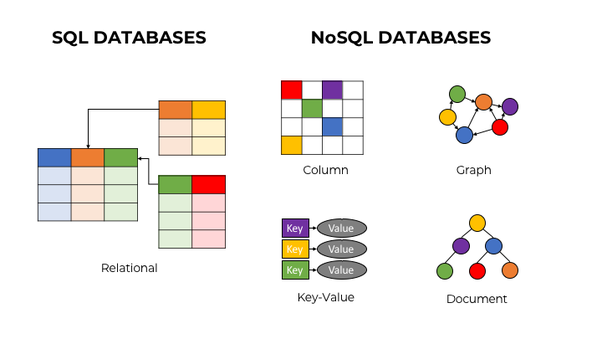
\includegraphics[width=\textwidth]{7design/images/nosqlDBs.png}
\caption{Comparison of the schema of SQL databases with the model of the four, categorised by Gupta et al., NoSQL database types \cite{Sahoo}.}
\label{fig:dbtypes}
\end{figure}

\paragraph{\gls{acid}} ACID describes four properties in the context of transaction processing. ACID properties guarantee data consistency and safe storage of the data \cite{Hauser} \cite{Foote}. However, ACID properties can hinder the scalability of a database, therefore many NoSQL systems use \gls{base} properties as an alternative \cite{Sundhara} \cite{Tang}. Brewer's \gls{cap} Theorem \cite{captheorem} \cite{Lynch} says that no distributed system can strongly and simultaneously guarantee consistency, availability and partition-tolerance (the ability of a cluster to function even when there is a break in communication between two nodes). Figure \ref{fig:cap} compares SQL and NoSQL databases using this theorem. Considering the CAP theorem, the preference is that the system favours consistency and availability over partition-tolerance. 

\FloatBarrier
\begin{figure}[H]
    \centering
    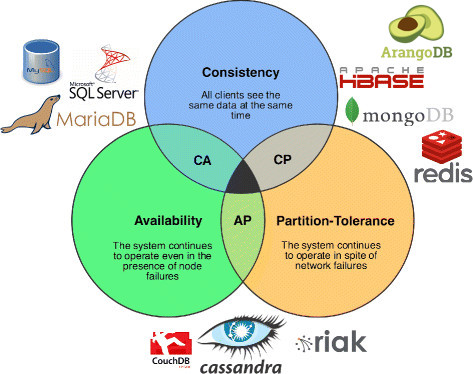
\includegraphics[width=10cm]{7design/images/capTheorem.jpeg}
    \caption{CAP Theorem for choosing NoSQL DB. Adapted from the diagram by Lourenço et al\cite{cap}.}
    \label{fig:cap}
\end{figure}

For codeHelper, SQL was selected. The small scale of the system, data and data variety (therefore resulting tables) meant that performance be unlikely to be affected to any noticeable extent. 

One of the key advantages of NoSQL is that it can store unstructured or semi-structured data. In codeHelper, the data is expected and required to have a rigid and predetermined structure. Traditional relational databases require and enforce data structure using the ACID properties, therefore improving the data integrity of the project. 



